%%%% fs-run-time-data-flow  FlameStream data flow

\label {fs-model}
\subsection{Data flow}

The top level of our data flow abstraction is a {\it stream}. Stream is represented by an ordered unlimited sequence of data items. Data item is a {\it payload} and a {\it meta-data} associated with it. 

\[DataItem := (Payload, Meta)\]

Payload is an arbitrary user-provided data. Meta-data is a structured system-assigned information. The primary purpose of the meta-data is to impose the total order on data items. 

Data payloads are got into the stream through {\it front} and got out through {\it barrier}. Particularly, front creates data items from input payloads by assigning them meta-data. Inside stream, data items can be dropped or their payloads and metas can be transformed. Eventually, barrier removes meta-information and outputs back pure payloads. High-level view of our stream is shown on the figure~\ref{stream}.

\begin{figure}[htbp]
  \centering
  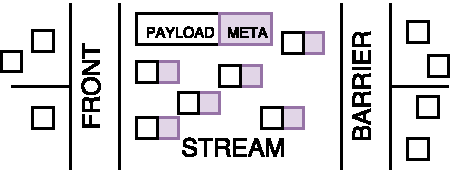
\includegraphics[width=0.48\textwidth]{pics/stream}
  \caption{Data flow}
  \label {stream}
\end{figure}

\subsection{Computaion flow}

The stream between front and barrier is handled by a directed data flow graph. Each node of the graph represents a single operation, which can have multiple inputs and outputs. Edges indicate the order of these operations. Data items are processed one-by-one in a "streaming" manner. The figure~\ref{logical-graph-figure} shows the example of data flow graph.

Our model allows cycles in the graph while data flow graphs are commonly assumed to be acyclic (DAGs) 
~\cite{Zaharia:2016:ASU:3013530.2934664, Carbone:2017:SMA:3137765.3137777}. Moreover, as we show further, there are cases when cycles are required, e.g. for MapReduce-based algorithms. 

\subsection{Physical deployment and partitioning}
Data flow graph is distributed among computation unit. Each computational unit in our runtime runs a process called {\it worker}, and each worker executes complete data flow graph. Every worker is assigned by an integer interval. Intervals are not intersected and cover the range of 32-bit signed integer.

Each input of an operation is assigned by the user-provided hash function called {\it balancing function}. This function is applied to the payload of data items and determines partitioning. Data items are repartitioned before each operation. After that, the corresponding data item is sent to the worker, which is responsible for the computed value. Therefore, load balancing explicitly depends on the balancing functions of the operations. The balancing functions are the part of business logic because optimal balancing requires the knowledge of payload distribution. Possible partitioning of this graph on two nodes is shown on the figure~\ref{physical-graph-figure}.

\begin{figure}[htbp]
  \centering
  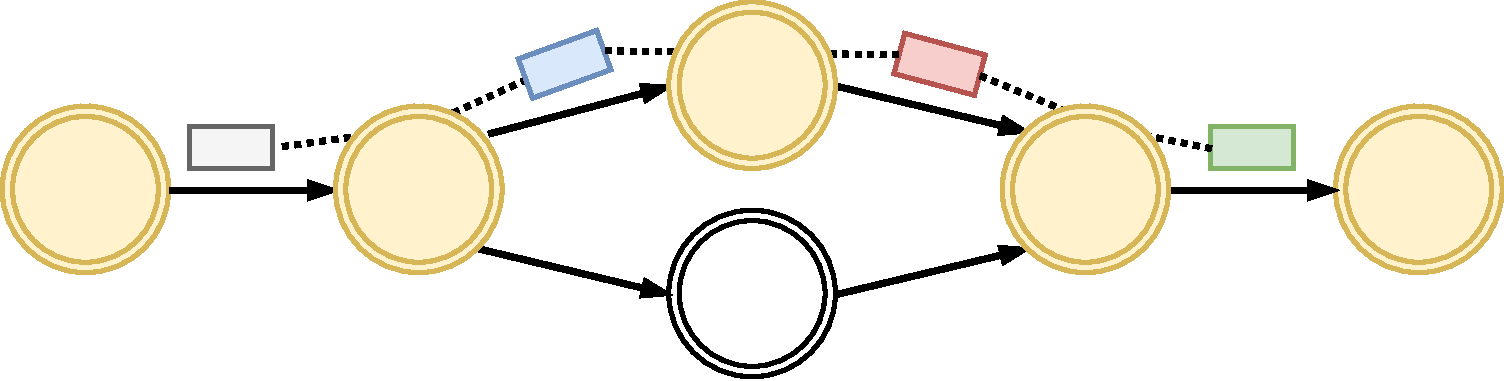
\includegraphics[width=0.48\textwidth]{pics/logical-graph}
  \caption{An example of the data flow graph}
  \label {logical-graph-figure}
\end{figure}

\begin{figure}[htbp]
  \centering
  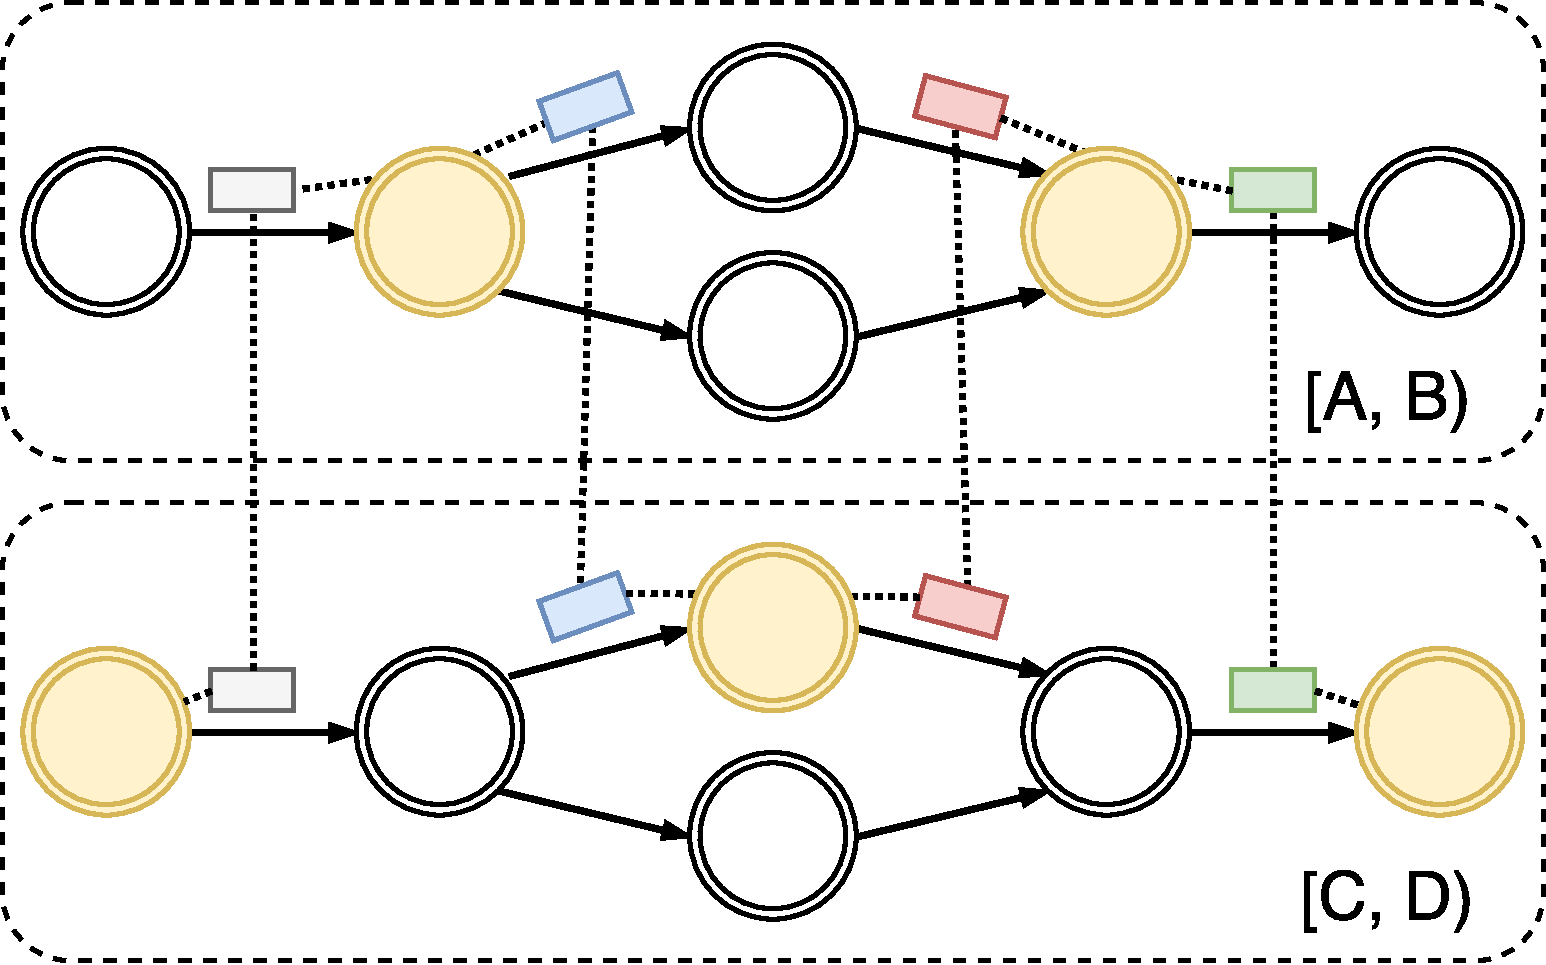
\includegraphics[width=0.48\textwidth]{pics/physical-graph}
  \caption{Possible partitioning of the data flow graph}
  \label {physical-graph-figure}
\end{figure}

\subsection{Ordering model}

As it was mentioned above, meta-information imposes an explicit total order on data items. Without diving into the details, it should be noted that the order of items is maintained across different fronts.

Let {\it image} be an output data item of an operation and {\it preimage} is a corresponding input item. In this terms, the order of images is preserved, i.e. the order of images is the same as the order of preimages. Moreover, the image of the item follows its preimage but precedes the next item. The concept of ordering is shown on the figure~\ref{ordering}

\begin{figure}[htbp]
  \centering
  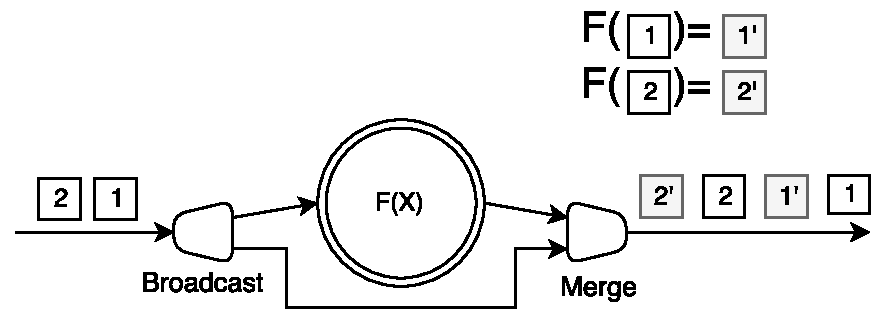
\includegraphics[width=0.30\textwidth]{pics/ordering}
  \caption{Ordering}
  \label {ordering}
\end{figure}

We assume that input items of the operations are strictly ordered. After the meta-data is assigned to the data item at the front, the rest of computations become deterministic.

\subsection{Operations}

The set of available operations is limited by the following list.

{\bf Map} applies a user-defined function to the payload of an input item. This function returns a sequence of data items with new payloads. An output sequence can be empty, in this case, the input item is filtered out.

{\bf Broadcast} replicates an input item to the specified number of operations or sinks. 

{\bf Merge} operation is initialized with the specified number of input nodes. Each input item from all inputs copied to the single output.

{\bf Grouping} has a {\it window size} parameter. Grouping stores input items in distinct buckets by the value of the input balancing function applied to the payload. When the next item arrives at the grouping, it is appended to the corresponding bucket according to the ordering model. Each time item grouping outputs window-sized {\it tuple item}, which consists of the last items of this bucket. The data items within tuple are ordered by the meta-information. If the size of the bucket is less than the window, all items of the bucket are taken. Grouping is the only operation that maintains state. To prevent collisions user can define equivalence relation to ensure that items with distinct payloads are got in the distinct buckets.

The following example illustrates the semantics of the operation. The grouping accepts items with payload represented as natural numbers: 1,2,3, etc. The hash function returns 1 if the number is even and 0 otherwise. If the window is set to 3, the output is:

\[(1), (2), (1|3), (2|4), (1|3|5), (2|4|6), (3|5|7), (4|6|8)...\]

The important property of the grouping is that the result is uniquely determined by the last element in the tuple. Therefore, grouping is the bijective mapping. Additionally, the results among items with different values of hash function are independent.

\subsection{User-defined parameters}

User is able to set up the following parameters:

\begin{enumerate}
  \item{Computation flow}
  \item{Balancing functions of the inputs}
  \item{Map functions}
  \item{Grouping windows}
\end{enumerate}

These parameters can produce more than one graph, which can yield equivalent results. Choosing among them is a performance optimization problem.    
It is important to mention, that there are no parameters for state-management. Therefore, business-logic is stateless. Nevertheless, the operations set is enough to implement any MapReduce transformation.

\subsection{MapReduce transformations on stream}

In this section, we demonstrate possible implementation of MapReduce-like transformation on a stream in order to show the soundness of our model. Map stage can be formulated in terms of our map operation. However, it is not obvious how to implement reduce stage, because it requires an explicit state handling. The algorithm~\ref{reduce} shows a generic reduce stage. The accumulator is an explicit state that should be maintained between subsequent iterations.

\begin{algorithm}
\caption{Generic reduce stage}
\label{reduce}
\begin{algorithmic}
  \Function{reduce}{$key$, $values$}
    \State $accumulator$ \Comment{reduce's state}
    \ForAll{$v \in values$} 
      \State \Call{combine}{$v$, $accumulator$}
    \EndFor
    \State \Return{$accumulator$}
  \EndFunction
\end{algorithmic}
\end{algorithm}

One possible way to implement reduce stage in our model is to make business logic state a part of the stream and work with it like with an ordinary data item. The figure~\ref{mapreduce-graph-figure} shows a generic graph for MapReduce computation. Map and reduce parts are highlighted with a dashed line.

\begin{figure}[htb]
  \centering
  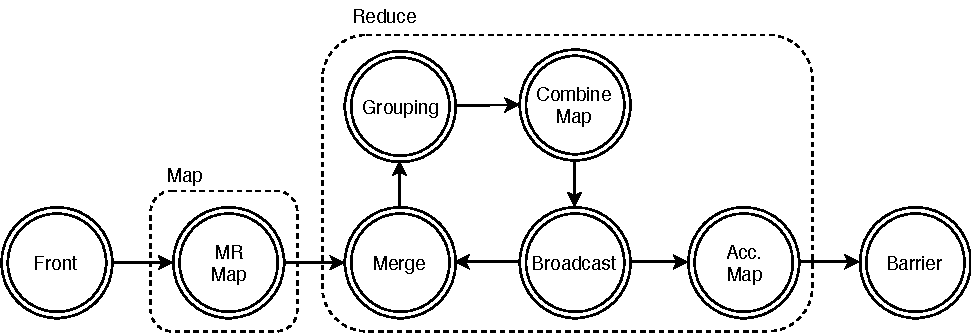
\includegraphics[scale=0.5]{pics/mapreduce}
  \caption{Logical graph for MapReduce transformations}
  \label {mapreduce-graph-figure}
\end{figure}

There are three types of data items in this stream: {\it input}, {\it mapped}, and {\it reduced} items. Mapped and reduced items have the key-value structure of a payload. The operations of the stream have the following purposes:

\begin{itemize}
  \item The first map operation accepts input items and outputs mapped items according to map stage of MapReduce model.
  \item The window of grouping is set to 2. It is used to group current reduce state with next data item in order to combine them together further. The hash function is designed to return distinct values for payloads with distinct keys.
  \item The second map implements the actual combining. It accepts inputs that have a form of: \textit{(mapped item)} or \textit{(reduced item, mapped item)}. The first kind is transformed into some initial value. The second one is combined into the reduce item as specified by reduce stage of MapReduce. The tuples with structure \textit{(mapped item, reduced item)} are filtered out.
  \item Broadcast operation is used to return the actual reduced item back to the grouping and, at the same time, to output it from the stream. 
\end{itemize}

The key idea is that ordering assumptions about data items guarantees that each reduced item always arrives at grouping right after previous mapped item and before a new one. Hence, each mapped item that has not been combined yet would be grouped with the right reduced item. Additionally, when combine map accepts tuple {\it (mapped item, reduced item)}, then it means that mapped item was generated before reduced, and therefore, it had been already combined. The cycle gives the ability for new reduced items to get back in grouping operation. Thereby, the stream reacts to each input item by generating new reduced item, which contains the actual value of the reduce stage.

We illustrate the MapReduce algorithm with an example of word counting. Map stage of this algorithm transforms each input word into key-value pair where the word is a key, and the value is 1. Reduce stage sums all values into the final result for the specific key. 

The example of input/output items, which are generated/ transformed by the part of the logical graph, is shown on the figure~\ref {word-count-figure}. According to our graph for MapReduce transformations, the item {\it m[dog, 1]} represents mapped item with key "dog" and value 1. The item {\it r[dog, 1]} describes reduced item with key "dog" and value 1. The figure shows how the model reacts on two consequent input items containing word "dog". The meta-information of items is omitted for simplification. More precisely, there are 4 stages separated by dotted lines:

\begin{enumerate}
    \item New mapped item with key "dog" arrives at grouping with an empty state. Grouping outputs tuple with this single item. Combine map transforms it to the first reduced item for key "dog" and value 1.
    \item The reduced item arrives at grouping after it went through the cycle. It is grouped in the tuple with the mapped item that has been already in the state with key "dog". However, combine map drops this tuple, because of the order of items.
    \item New mapped item with key "dog" arrives at grouping. It is inserted right after the reduced item in the bucket for key "dog". The grouping operation outputs tuple containing the reduced item and new mapped item. Map operation combines reduced and mapped items into new reduced items with key "dog" and value 2.
    \item New reduced item arrives at grouping through the cycle, but new generated tuple is not accepted by combine map, as well as in step 2.
\end{enumerate}

\begin{figure}[htb]
  \centering
  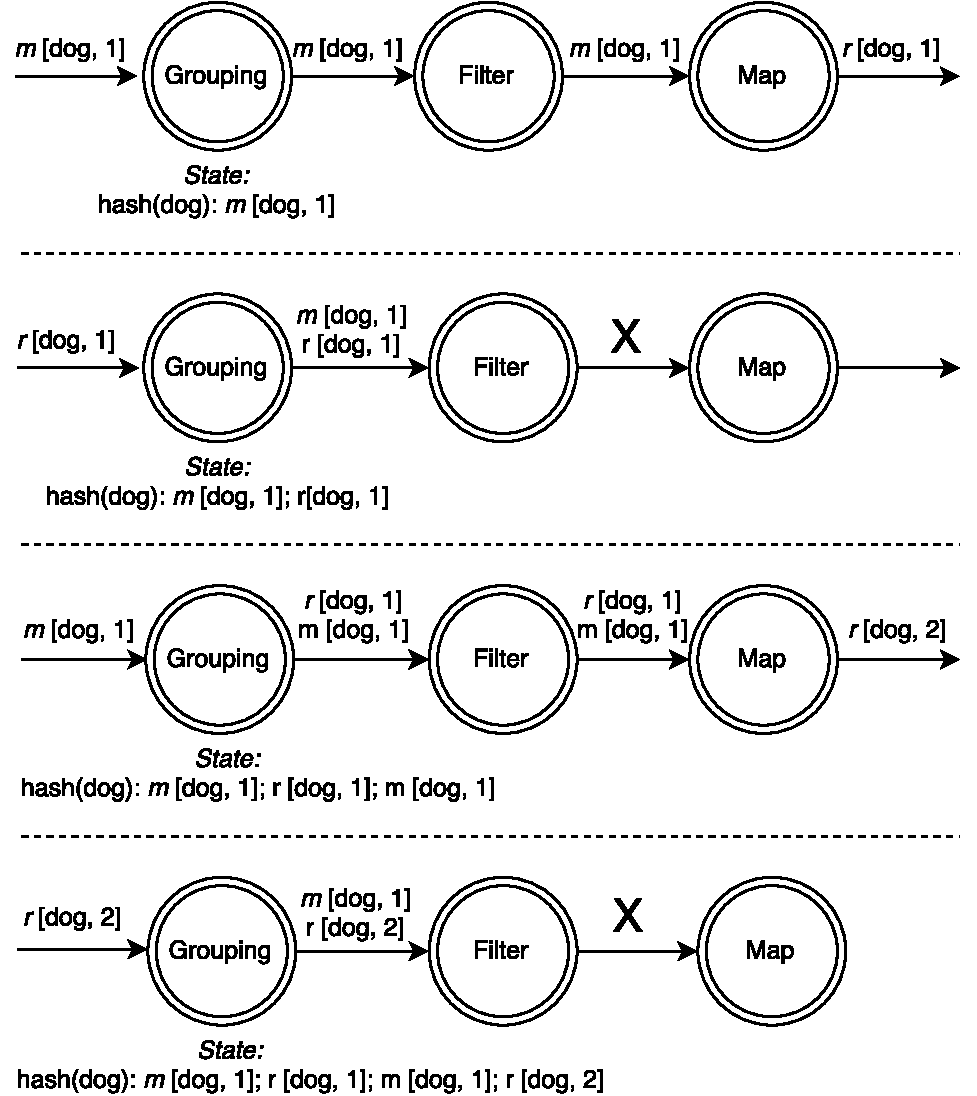
\includegraphics[scale=0.5]{pics/wordcount}
  \caption{Part of the stream evalutaion for word counting}
  \label {word-count-figure}
\end{figure}
